\documentclass[runningheads,a4paper]{llncs}

\usepackage{amssymb}
\setcounter{tocdepth}{3}
\usepackage{graphicx}
\usepackage{url}
\urldef{\mailsa}\path|{pjan520, cchatfield, sharris, rhua440, yhunter, samli, rogerl, rdro117,tehbelinda, bradh, bernhardh, morri, claude}@cse.unsw.edu.au|
\newcommand{\keywords}[1]{\par\addvspace\baselineskip
\noindent\keywordname\enspace\ignorespaces#1}

\begin{document}

\mainmatter 

\title{
Team rUNSWift\\
University of New South Wales, Australia\\
\vspace{1cm}
RoboCup 2012\\
Standard Platform League}
\titlerunning{RoboCup 2012 rUNSWIFT}

\author{
Peter Anderson
\and Carl Chatfield
\and Sean Harris
\and Richard Hua
\and Youssef Hunter
\and Sam Li
\and Roger Liu
\and Ritwik Roy
\and Belinda Teh
\and Brad Hall
\and Bernhard Hengst
\and Maurice Pagnucco 
\and Claude Sammut
\mailsa\\
}
\authorrunning{Anderson, et. al.}

\institute{
School of Computer Science and Engineering\\
University of New South Wales\\
Sydney 2052 Australia\\
\url{http://www.cse.unsw.edu.au}}

\maketitle

\begin{abstract}
RoboCup continues to inspire and motivate our research interests in cognitive robotics and machine learning, including vision, state-estimation, locomotion, layered hybrid architectures, and high-level programming languages. The 2012 rUNSWift team consists primarily of final year undergraduate students under the supervision of  leaders who have been involved in RoboCup for many years. Major developments in 2012 include porting previous code to the new Nao V4 - RoboCup Edition humanoid robot from Aldebaran-Robotics. Innovation in vision, localisation, motion, behaviour, and the supporting software infrastructure and tools has been aided by the upgraded cameras and faster the processor in the new Nao.   
\end{abstract}

%\begin{figure} [t]
%\centering
%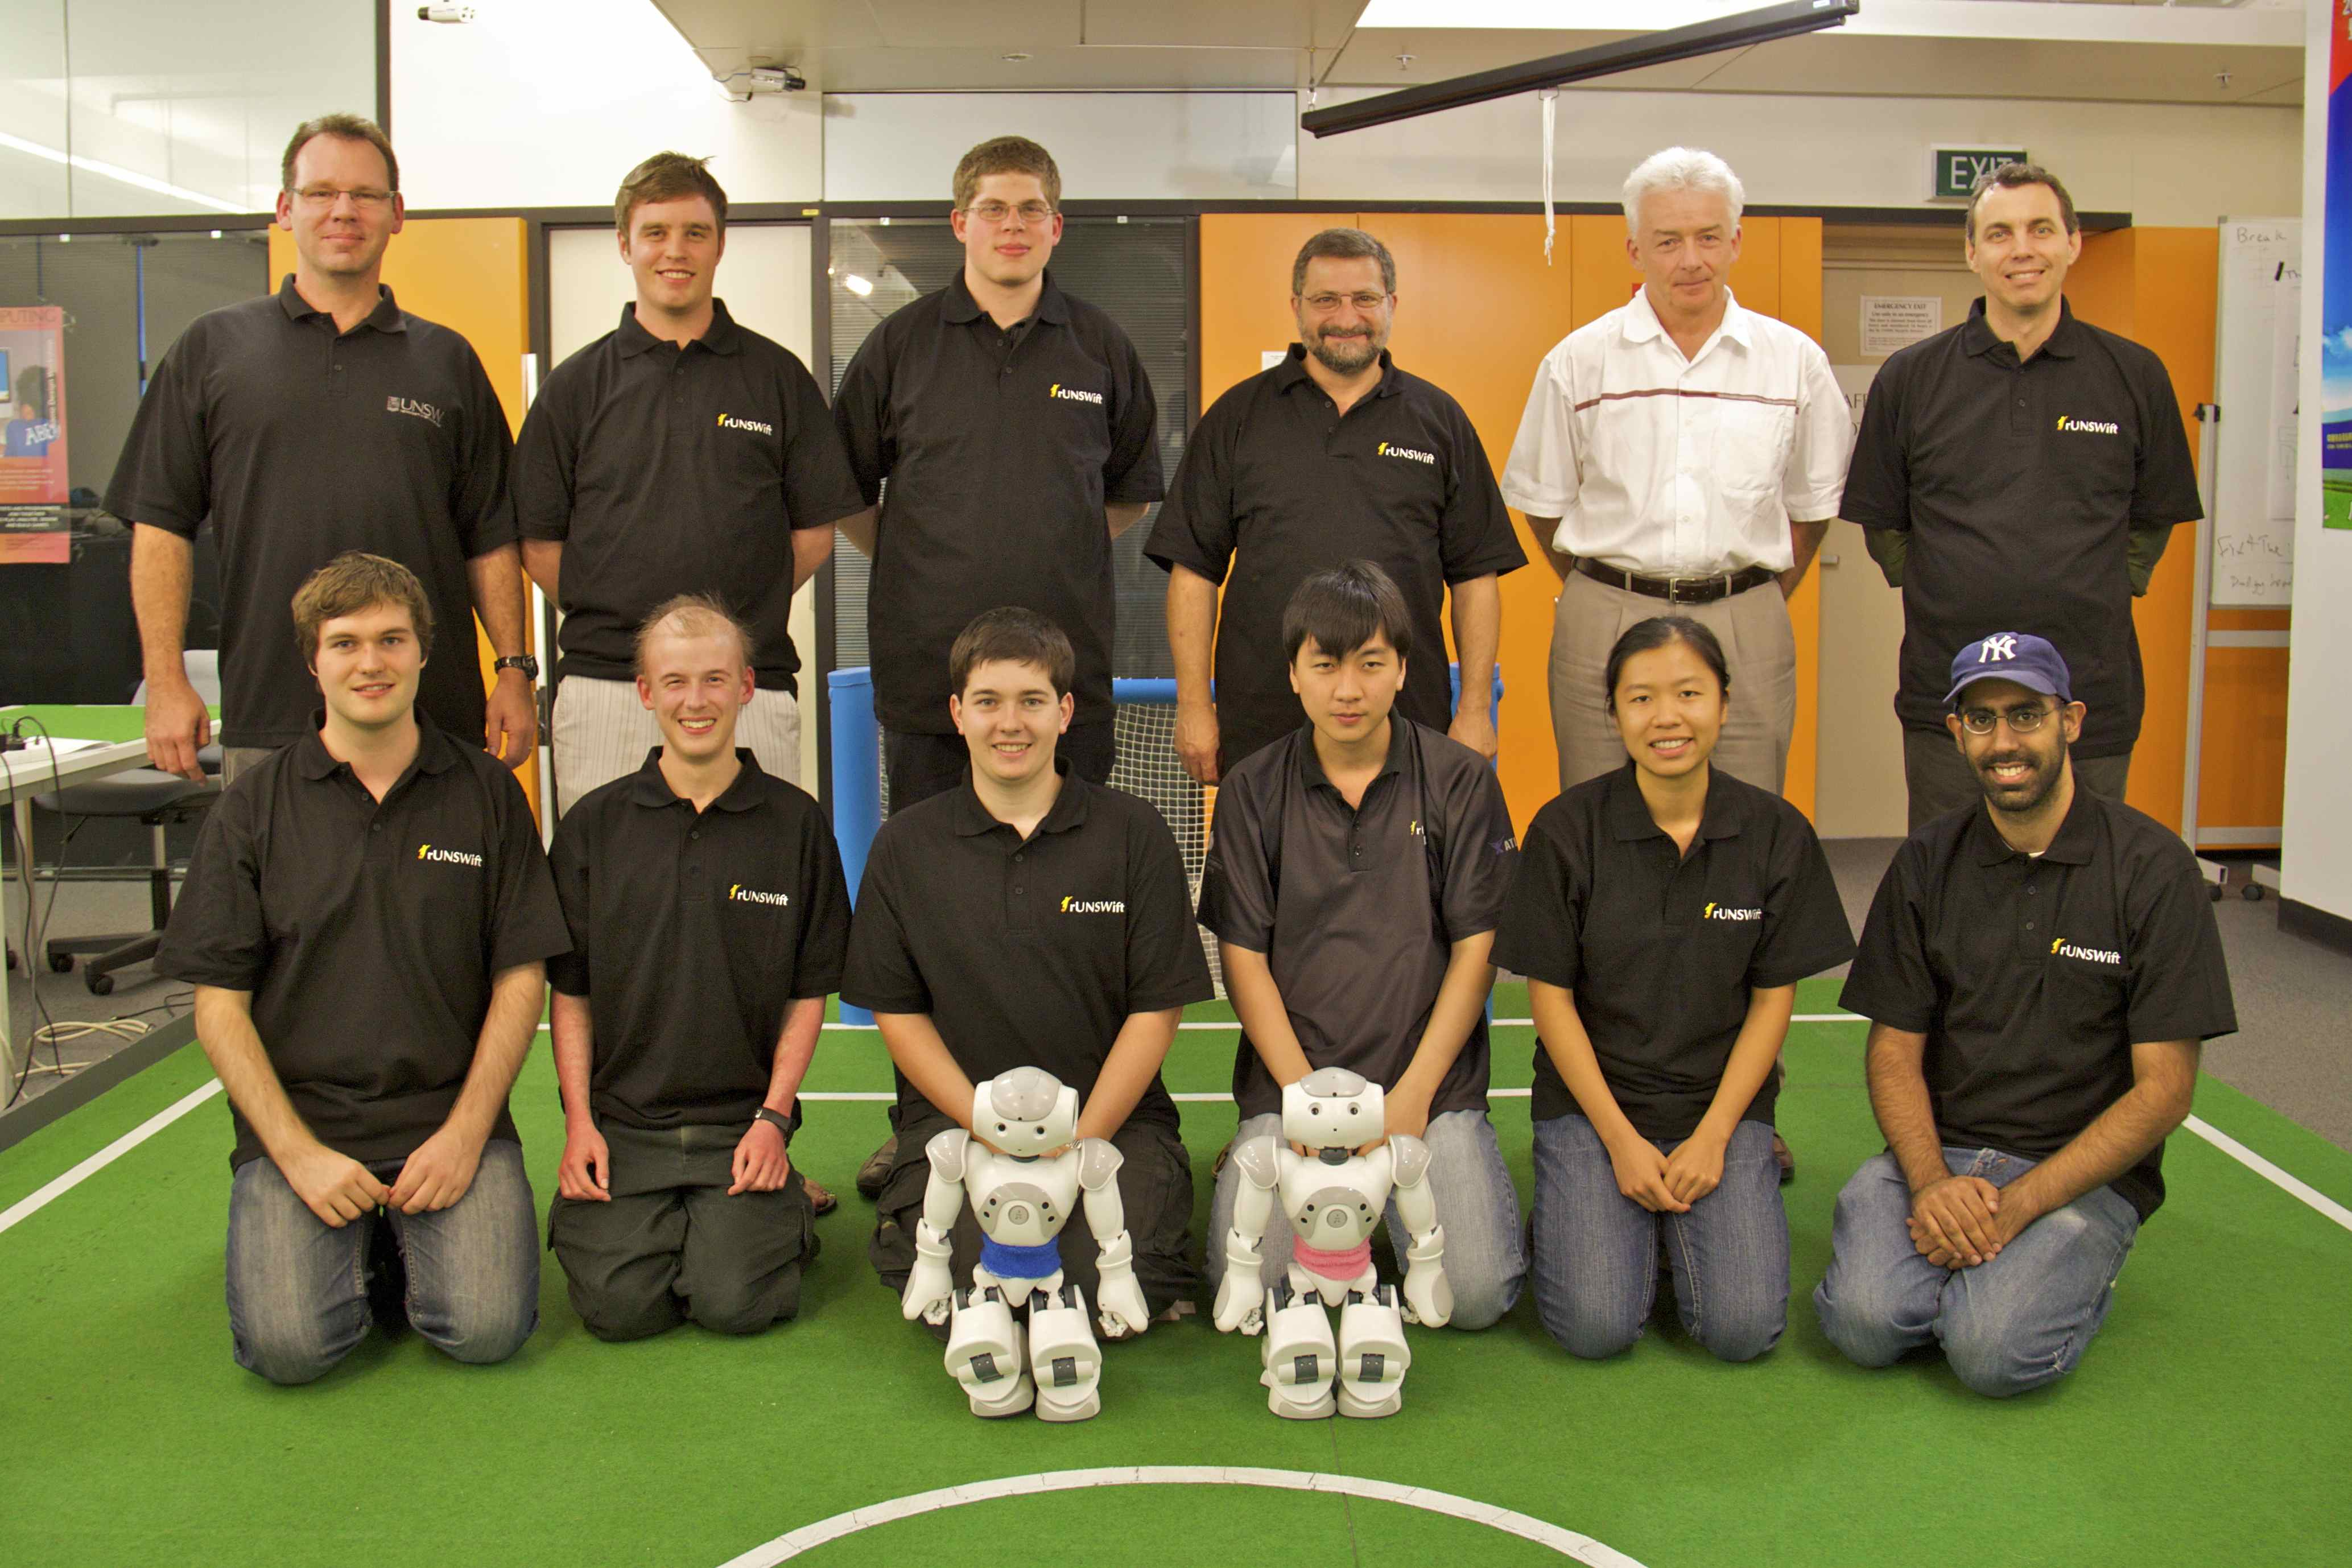
\includegraphics[width=1.0\textwidth]{TeamPic.jpg}
%\caption{\textit{The 2011 rUNSWift Team. Top: Claude Sammut, Bernhard Hengst, Carl Chatfield, Brad Hall, Maurice Pagnucco. Middle: Jayen Ashar, 
%David Claridge, Brock White, Jimmy Kurniawan, Youssef Hunter. Bottom: 
%Sean Harris, Belinda Teh, Yongki Yusmanthia, Hung Nguyen.}} \label{fig-team}
%\end{figure}

\section{The Team}
The RoboCup Standard Platform League (SPL) has been and continues to be excellent training for the students who also make a significant contribution towards research. The UNSW SPL teams have largely been made up of final-year undergraduate students, supported by faculty and research students. The 2012 rUNSWift team includes undergraduate students: Peter Anderson, Carl Chatfield, Richard Hua, Youssef Hunter, Sam Li, Roger Liu and Belinda Teh; postgraduate students Sean Harris and Ritwik Roy; faculty staff: Bernhard Hengst, Maurice Pagnucco and Claude Sammut; and Development Manager Brad Hall. %Some of the team members are a pictured in Figure \ref{fig-team}.

The team has the financial support of the School of Computer Science and Engineering at the University of New South Wales.  The School provides considerable organisational support for travel. We have a competition standard field and a wealth of experience from our participation in the standard platform league (previously Sony four-legged league), simulation, and rescue competitions. 

A UNSW team has taken part in every RoboCup competition since 1999. In the following sections we describe our broader research interests and list our contributions over the years. Team reports, code and videos are available at internet address: \url{http://www.cse.unsw.edu.au/help/students/robocup}.

\section{Research Interests}

The vision of many robotics researchers is to have machines operate in unstructured, real-world domains. Our long-term aim is to develop general-purpose intelligent systems that can learn and be taught to perform many different tasks autonomously by interacting with their environment. As an approach to this problem, we are interested in how machines can compute abstracted representations of their environment through direct interaction, with and without human assistance, in order to achieve some objective. These future intelligent systems will be goal directed and adaptive, able to program themselves automatically by sensing and acting, and accumulating knowledge over their lifetime.  

The School of Computer Science and Engineering at the University of New South Wales is arguably the premiere Australian computing school. UNSW is the only Australian university ranked among the top 100 for Computer Science in the Academic Ranking of World Universities (\url{http://www.arwu.org}). Autonomous Systems is a priority research area for UNSW. Our general research focus, of which the RoboCup SPL is a part, is to:
\begin{itemize}
\item further develop reasoning methods that incorporate uncertainty and real-time constraints and that integrate with the statistical methods used in SLAM and perception
\item develop methods for using estimates of uncertainty to guide future decision making so as to reduce the uncertainty 
\item extend these methods for multi-robot cooperation
\item use symbolic representations as the basis for human-robot interaction
\item develop learning algorithms for hybrid systems, such as using knowledge of logical constraints to restrict the search of a trial-and-error learner and learning the constraints
\item develop high level symbolic robotic languages that provide abstractions for a large range of deliberation, planning and learning techniques so as to simplify robot programming
\end{itemize}


\section{rUNSWift 2012 Robotic Architecture} \label{sectionRoboticArchitecture2011}

The rUNSWift robotic architecture [1] is a task-hierarchy for a multi-agent team of four Naos. We use a fault-tolerant network-centric architecture. This means that each robot may have a slightly different view of the world and therefore of its role on the team. The approach has the advantage of providing some redundancy in case individual robots are disqualified or stop working.

Starting at the root-level the game-controller invokes the high-level states for playing soccer. At lower levels, the walk generators execute temporally extended walk phases that invoke primitive state transitions constituting the motion of the robot as it transitions between poses 100 times each second. 

\begin{figure}[!htp]
\centering
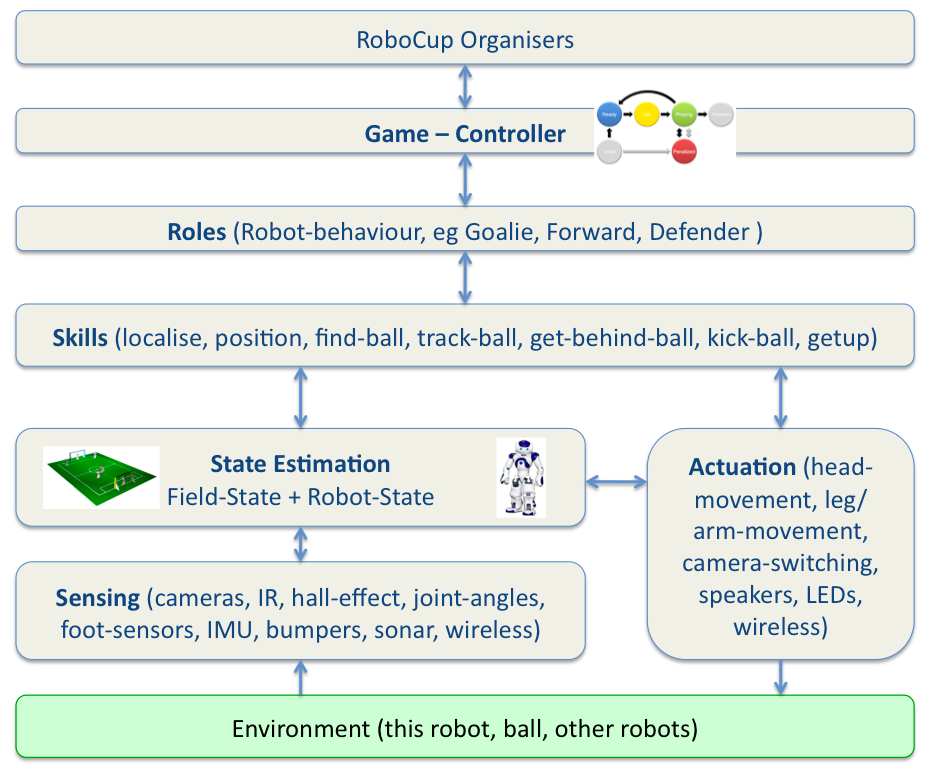
\includegraphics[width=1.0\textwidth]{runswift2011architecture}
\caption{The 2012 UNSW SPL robotic architecture.} \label{figrunswift2011architecture}
\end{figure}

\subsection{Vision}
Our vision system evolved significantly over the last fourteen years. From the beginning, in 1999, we used a simple learning system to train the colour recognition system. In 2001, we used a standard machine learning program, C4.5, to build a decision tree recogniser. This turned out to be very important since the lighting we encountered at the competition was very different from our lab and our previous vision system was not able to cope. Also in 2000, our vision system became good enough to use robot recognition to avoid team mates (Sammut \& Hengst, 2003). 

In recent years, we have updated the vision system to recognise the field-boundary, field-markings and to rely less on colour by using edge-features. We have also introduced a foveated vision system and virtual saccades to maximise scare computational resources. With the final removal this year of any specified landmark that allows the determination of target goal direction (both goals are now coloured yellow) we will for the first time use a natural landmark recognition algorithm that is able to localise the robot in real-time. This tailored SLAM approach, based on one-dimensional local image features, is the subject of a paper to appear at the 2012 RoboCup Symposium (Anderson, et al, 2012). Spin-offs include visual odometry and slip-detection. 

\subsubsection{Localisation}
The 2000 competition saw the initial use of a Kalman filter-based localisation method that continued to evolve in subsequent years (Pham et al, 2002). In the 2000 competition, advantages in localisation and locomotion meant that the team never scored less than 10 goals in every game and only one goal was scored against it in the entire competition. Starting from a simple Kalman filter in 2000, the localisation system evolved to include a multi-modal filter and distributed data fusion across the networked robots. In 2006, we went from treating the robots as individuals sharing information, to treating them as one team with a single calculation spread over multiple robots.  This allowed us to handle multiple hypotheses.  It also allowed us to use the ball for localisation information. 

Including more and more robots in the one Kalman filter does not scale easily because the number of modes grows exponentially. We are now experimenting with multi-robot-multi-modal Kalman filtering and researching the application of loopy belief revision to achieve similar benefits more efficiently with larger teams. A significant innovation in 2012 is the use of a variation of the Iterative Closest Point  (ICP) algorithm extending previous work on field-line matching (Sheh \& Hengst, 2004; Ratter, 2011) to other visual features and objects. This novel algorithm will be described in rUNSWift technical reports by Anderson \& Hunter later this year. 

\subsubsection{Locomotion}
In 2000, we introduced the UNSW walk, which became the standard across the league (Hengst et al, 2002). The key insight was to describe the trajectory of the paws by a simple geometric figure that was parameterised. This made experimentation with unusual configurations relatively easy. As a result, we were able to devise a gait that was much faster and more stable than any other team. Almost all the other teams in the 4-legged league at the time adopted a similar style of locomotion, some starting from our code. The flexibility of this representation led to another major innovation in 2003. We were the first team to use Machine Learning to tune the robot's gait, resulting in a much faster walk (Kim \& Uther, 2003). In succeeding years, several teams developed their own ML approaches to tuning the walk. Starting from the parameterised locomotion representation, the robots are able to measure their speed and adjust the gait parameters according to an optimisation algorithm.

Bipedal locomotion research in our group includes applications of Machine Learning to gaits. PhD student Tak Fai Yik (a member of the champion 2001 four-legged team) collaborated with Gordon Wyeth at the University of Queensland to evolve a walk for the GuRoo robot (Wyeth, et al, 2003), which was entered in the humanoid robot league. Our current research is directed towards  learning versatile bipedal locomotion controllers using hierarchical reinforcement learning techniques with continuous states and actions. It is well known that learning by sheer enumeration of problem variables does not scale. We are exploiting the structure of the walking domain to decompose the problem to learn near-optimal control solutions. The team was placed third in the SPL Open Challenge last year demonstrating the learning of ankle-tilt control for bipedal balancing and walking  (Hengst, et al, 2011).   

\subsubsection{Software Engineering and Architecture}
Throughout the software development of the Aibo code, we have adopted a modular, layered architecture. The lowest layers consist of the basic operations of vision, localisation and locomotion. The behaviours of the robots are also layered, with skills such as ball tracking, go to a location, get behind ball, etc, being at the lowest level of the behaviour hierarchy, with increasingly complex behaviours composed of lower-level skills. Originally, all the behaviours were coded in C/C++ but in 2005 and 2006, as in 2010 and 2012 the upper layers were replaced by Python code.  We have also experimented with higher level functions coded in the experimental cognitive robotics language Golog. 

One of the key reasons behind the UNSW team's success has been its approach to software engineering. It has always been: keep it simple, make the system work as a whole and refine only what evidence from game play tells us needs work. This practical approach has had a strong effect on our research because it has informed us about which problems are really worth pursuing and which ones are only imagined as being important.

\section{Participation and Performance}

A UNSW team has taken part in every RoboCup competition since 1999. Details of awards are as follows:

\subsubsection{Standard Platform League/Four-legged league: 1999-2006, 2008-2010}
\begin{itemize}
\item 1st place: 2000, 2001, 2003
\item 2nd place: 1999, 2002, 2006, 2010
\item 3rd place: 2005
\item Quarter-finalists: 2004, 2008, 2011
\item Challenges: 1st in 1999, 2000, 2001, 2002, 2010
\item Challenges: 2nd in 2003
\item Challenges: 3rd in 2011
\end{itemize}

\subsubsection{Simulation soccer: 2001 - 2003}
\begin{itemize}
\item 7th place: 2002
\end{itemize}

\subsubsection{Rescue: 2005 - 2007, 2009-2010}
\begin{itemize}
\item 3rd overall: 2005
\item Semi-finalists and 2nd in autonomous robot challenge: 2006
\item Finalists: 2007, 2009. 
\item Best in class Autonomy: 2009, 2010, 2011 
\item 2nd in Mobility: 2009
\item Award for innovative user interfaces: 2009
\end{itemize}

\section*{References}

RoboCup SPL related publications:
\begin{enumerate}
\item Robot Localisation Using Natural Landmarks, Peter Anderson, Yongki Yusmanthia, Bernhard Hengst, Arcot Sowmya, RoboCup Symposium, 2012
\item Fast Object Detection with Foveated Imaging and Virtual Saccades on Resource Limited Robots, Adrian Ratter, David Claridge, Jayen Ashar and Bernhard Hengst, The 24th Australasian Joint Conference on Artificial Intelligence (AI2011), 2011
\item Learning Ankle-Tilt and Foot-Placement Control for Flat-footed Bipedal Balancing and Walking, Bernhard Hengst, Manuel Lange, Brock White, Humanoids, Bled, Solovinia, 2011
\item RoboCup Standard Platform League - rUNSWift 2010, Jayen Ashar, David Claridge, Brad Hall, Bernhard Hengst, Hung Nguyen, Maurice Pagnucco, Adrian Ratter, Stuart Robinson, Claude Sammut, Benjamin Vance, Brock White, Yanjin Zhu, Australasian Conference on Robotics and Automation, Dec 1st-3rd Brisbane Australia, 2010
\item 2010 Team Report, Code and Videos http://www.cse.unsw.edu.au/~robocup
\item 1999--2009 team reports as well as selected code are available at URL:\\
\url{http://robocup.web.cse.unsw.edu.au}
\item Aaron James Soon Beng Tay (2009) Walking Nao Omnidirectional Bipedal Locomotion. UNSW SPL team report.
\item David G. Claridge, Carl Chatfield, Gary Huynh (2009). Software Systems for the Nao Humanoid Robot. UNSW SPL team report.
\item Mitchell Currie (2009) Robocup 2009: Localisation. UNSW SPL team report.
\item Brimo, A. (2008) RoboCup 2008. UNSW RoboCup 2008 Report.
\item Chen, S., Siu, L., Vogelgesang, T., Yik, T. F., Hengst, B., Pham, S. B. and Sammut, C. (2002). The UNSW RoboCup 2001 Sony Legged Robot Leage Team. In A. Birk, S. Coradeschi and S. Tadokoro (Eds.), RoboCup 2001: Robot Soccer World Cup V (pp. 39-48): Springer.
\item Chen, J., Chung, E., Edwards, R. \& Wong, N. (2003). Rise of the Aibos III - Aibo RevolutionsI. RoboCup Team Report. http://www.cse.unsw.edu.au/ ~robocup/2003site/report2003.pdf
\item Collien, D. and Huynh, G. (2008). From AIBO to NAO: The Transition from 4-Legged to 2-Legged Robot Soccer, UNSW RoboCup 2008 Report.
\item Hengst, B., Ibbotson, D., Pham, S. B. and Sammut, C. (2000). UNSW RoboCup 2000 Team Report. http://www.cse.unsw.edu.au/~robocup 
\item Hengst, B., Ibbotson, D., Pham, S. B., Dalgliesh, J., Lawther, M., Preston, P. and Sammut, C. (2001). The UNSW Robocup 2000 Sony Legged League Team. In P. Stone, T. Balch and G. Kraetzschmar (Eds.), Robocup 2000: Robot Soccer World Cup IV (Vol. 2019, pp. 64-75), Springer.
\item Dalgliesh, J. and Lawther, M. (1999). Playing soccer with quadruped robots. Computer Engineering Thesis, School of Computer Science and Engineering, University of New South Wales.
\item Hengst, B., Pham, S. B., Ibottson, D. and Sammut, C. (2002). Omnidirectional Locomotion for Quadruped Robots. In RoboCup 2001: Robot Soccer World Cup V (pp. 368-373). Berlin: Springer.
\item Kadous, M. W., Sheh, R. and Sammut, C. (2006). Controlling Heterogeneous Semi-autonomous Rescue Robot Teams. In 2006 IEEE International Conference on Systems, Man, and Cybernetic.
\item Kadous, W., Sammut, C. and Sheh, R. (2006). Autonomous Traversal of Rough Terrain Using Behavioural Cloning. In The 3rd International Conference on Autonomous Robots and Agents.
\item Kim, M. S. And Uther, W. (2003). Automatic gait optimisation for quadruped robots. In Australasian Conference on Robotics and Automation. Brisbane.
\item Levesque, H. J., and Pagnucco, M., (2000) Legolog: Inexpensive Experiments in Cognitive Robotics, In Proceedings of the Second International Cognitive Robotics Workshop, Berlin, Germany.
\item Pagnucco, M. and Rajaratnam, D. (2005): Inverse Resolution as Belief Change. IJCAI 2005.545.
\item Pham, K. C. and Sammut, C. (2005). RDRVision - Learning vision recognition with Ripple Down Rules. Proc. Australasian Conference on Robotics and Automation (pp. 7 pages).
\item Pham, S. B., Hengst, B., Sammut, C. and Ibbotson, D. (2002). Stochastic Gradient Descent Localisation in Quadruped Robots. In RoboCup 2001: Robot Soccer World Cup V (pp. 447-452). 
\item Nardi, D., Riedmuller, M. and Sammut, C. (Eds.). (2005). Proc of the RoboCup 2004 Symposium.
\item Sammut, C. and Hengst, B. (2003). The Evolution of a Robot Soccer Team. Robotics Research: The Tenth International Conference (pp. 517-529): Springer.
\item Sammut, C. (2003). Robot Soccer: Science or just fun and games? Proceedings of the Australian Joint Conference on Artificial Intelligence (pp. 12-23). Perth: Springer.
\item Sammut, C., Kadous, W., \& Sheh, R. (2007). In K. Furukawa (Ed.), Learning to Drive Over Rough Terrain International Symposium on Skill Science, Tokyo.
\item Sheh, R., Kadous, M.W., Sammut, C., \& Hengst, B. (2007). In D. Nardi (Ed.), Extracting Terrain Features from Range Images for Autonomous Random Stepfield Traversal. IEEE International Conference on Safety, Security and Rescue Robotics, Rome.
\item Raymond Sheh, Bernhard Hengst (2004). A Fast Vision Sensor Model: Matching Edges with NightOwl Proceedings of the Australasian Conference on Robotics and Automation (ACRA)
\item Tay, A. (2008). Exploration of Nao and its Locomotive Abilities. UNSW RoboCup 2008 Report.
\item Thomas J., Blair, A. \& Barnes, A., (2003). Towards an efficient optimal trajectory planner for multiple mobile robots, Proc. 2003 International Conference on Intelligent Robots and Systems.
\item Wyeth, G., Kee, D. and Yik, T. F. (2003). Evolving a Locus Based Gait for a Humanoid Robot. In International Conference on Robotics and Intelligent Systems. Las Vegas.
\item Yik, T. F. (2007).  Locomotion of Bipedal Robots: Planning and Learning to Walk. PhD Thesis. School of Computer Science and Engineering, University of New South Wales.
\item Yik, T.F., \& Sammut, C. (submitted). In M. Srinivasan \& M. Dunbabin (Eds.), Trial-and-Error Learning of a Biped Gait Constrained by Qualitative Reasoning. Australasian Conference on Robotics and Automation, Brisbane.
\item Zheng Wang, Bernhard Hengst, Claude Sammut (2002). Localisation in an Uncertain World with Multiple Agents, MI19.
\end{enumerate}

\end{document}
